\documentclass[dvisvgm,tikz,border=4pt]{standalone}
\usepackage{amsmath,amssymb}

\usetikzlibrary{arrows.meta,positioning,automata,shapes,shapes.misc,calc,decorations.pathmorphing,decorations.markings,angles,quotes,patterns,mindmap,matrix,knots,hobby,trees}
\tikzset{->-/.style={decoration={markings, mark=at position 0.5 with {\arrow{Stealth}}}, postaction={decorate}}}
\begin{document}
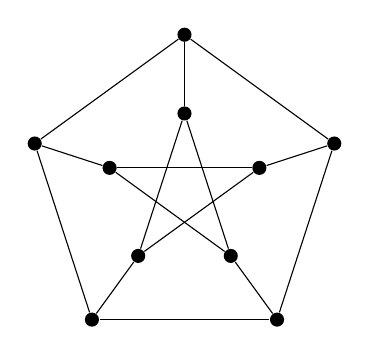
\begin{tikzpicture}[every node/.style={circle, fill=black, inner sep=1.8pt}]
\foreach \i in {0,...,4} {
  \node (o\i) at ({90+72*\i}:2) {};
  \node (i\i) at ({90+72*\i}:1) {};
}
\foreach \i [evaluate=\i as \j using {int(mod(\i+1,5))}, evaluate=\i as \k using {int(mod(\i+2,5))}] in {0,...,4} {
  \draw (o\i) -- (o\j);
  \draw (o\i) -- (i\i);
  \draw (i\i) -- (i\k);
}
\end{tikzpicture}
\end{document}
